\sectionlink{非相対論的フェルミオンのEFT}


\subsectionlink{真空中の非相対論的フェルミオン} \label{sec: NR fermions in vacuum}

\ref{sec: toy model}節のトイモデルでは、フェルミオンが相対論的、すなわちエネルギーが$E \gg m c^2$であったため、パワーカウンティングは特に容易であった。\footnote{この節では、$c$の因子をすべて復活させる。特に、$\d_0 = \d_t / c$である。}その結果、$\Psi$に作用する偏微分の各成分はすべて同じように、すなわち$\d_\mu \sim E /c$とスケールした。しかし、運動量が$p \ll mc$である非相対論的フェルミオンの散乱過程では、もはやこれは成り立たない。この場合は
%
\begin{align}
	\d_\mu \Psi \sim i \, (- m c, \, \vec p \, ) \, \Psi,
\end{align}
%
であり、第0成分は空間成分よりもはるかに大きくなる。明確にしておくと、微分によってスケーリングが異なること自体が必ずしも問題なのではない。後に見るように、これは多くのEFTで起こる。ここでの問題は、第0成分がフェルミオンの運動量、あるいは同じことだがエネルギーに応じてまったくスケールしないことである。このため、$\Psi$の高階時間微分は低エネルギーで必ずしもより強く抑制されず、したがってLagrangianの演算子は運動量のべきに従って明確には整理されない。幸い、次の\high{位相の再定義}によって新しい場$\tilde \Psi$を導入すれば、この問題は容易に解決できる。
%
\begin{align} \label{Psi tilde def vacuum}
	\Psi (t, \vec x)  \equiv e^{- i m c^2 t} \tilde \Psi (t, \vec x) 
\end{align}
%
すると、$\tilde \Psi$の微分は
%
\begin{align} \label{Psi tilde derivatives}
	\d_\mu  \tilde \Psi = \d_\mu \left( e^{i m c^2 t} \Psi \right) \sim i \, (- \frac{p^2}{2mc}, \, \vec p \, ) \, \tilde \Psi
\end{align}
%
とスケールする。したがって、微分を余分に含む演算子は、運動量が有効理論の強結合スケールに比べて小さいとき、より強く抑制される。

この場の再定義をLagrangianの段階で直接実行してみることは有益である。例えば、式\eqref{4pt tree effective theory}の作用で$(\bar  \Psi \gamma^5 \Psi)^2 \to (\bar  \Psi  \Psi)^2$としたものを考えよう。$c$のべきとガンマ行列をすべて明示すれば、作用を$\tilde \Psi$によって直接、次のように書ける。
%
\begin{align} \label{4pt tree effective action with c}
	S_{\rm eff} = \int dt \, d^3 x \, c \left\{ \tilde \Psi^\dag \l[ \frac{ i \d_t}{c}  +  i \gamma^0 \gamma^i \d_i +  (1 - \gamma^0) m c  \r] \tilde \Psi - \frac{y^2}{2 M^2c} (\tilde \Psi^\dag \gamma^0 \tilde \Psi )^2\right\} \ .
\end{align}
%
4次相互作用の前の$1/c$という因子は、結合定数を再定義すれば常に吸収できるが、後の便宜のために導入してある。$\tilde \Psi$の微分に対するパワーカウンティング則\eqref{Psi tilde derivatives}によれば、角括弧内の支配的な項は$m c$に比例する項である。このことから、射影行列\footnote{$P_\pm$が実際に射影演算子の定義を満たすこと（$P_\pm^2 = P_\pm$）は容易に確かめられる。さらに、これらは互いに直交し（$P_+ P_- = P_- P_+ = 0$）、完全系をなす（$P_+ + P_- = 1$）。}$P_\pm \equiv \tfrac{1}{2} (1 \pm \gamma^0)$を導入して、$\tilde \Psi$を$\tilde \Psi_\pm \equiv P_\pm \tilde \Psi$の和に分解するのが自然である。Lagrangianの主要な2次項は$mc^2  \tilde \Psi_+^\dag \tilde \Psi_+$なので、この非相対論的EFTの展開パラメータである$p/mc$について摂動的に計算することにより、$\tilde \Psi_+$を積分消去し、$\tilde \Psi_-$だけの有効Lagrangianを得ることができる。非相対論的粒子では$p = m v$なので、この展開パラメータは$v /c$とも表せることに注意しよう。
%
\begin{eBox}
%
{\bf 演習4.1：}$\tilde \Psi_+$をツリーレベルで積分消去し、$p/mc$の最低次で$\tilde \Psi_-$の有効作用を導け。
%
\end{eBox}

物理的には、非相対論的領域でモードの半分を積分消去できるのは、例えば粒子だけが関与する低エネルギー散乱では、エネルギー保存により反粒子を生成できないからである。$\gamma^0$が対角的となるDirac行列のDirac表示~\cite{Zee:2003mt}を用いれば、このことをより明示的に示せる。\footnote{非相対論的極限では、この基底は文献~\cite{Srednicki:2007ab}で用いられている、$\gamma^5$が対角的となるWeyl基底よりも便利である。二つの基底におけるスピノルは、$S = \frac{1}{\sqrt{2}} \left( \begin{smallmatrix} 1 & 1 \\ -1 & 1 \end{smallmatrix} \right)$とした線形変換$\Psi_{\rm Dirac} = S \, \Psi_{\rm Weyl}$によって結び付いている。}
%
\begin{align} \label{2-spinor def}
	\gamma^0 = \begin{pmatrix}
		1 &  0 \\ 0 & -1 
	\end{pmatrix} \qquad \Longrightarrow \qquad \tilde \Psi_- = \begin{pmatrix}
		0 \\ \psi 
	\end{pmatrix} .
\end{align}
% 
このとき、2成分スピノル$\psi$に対する最低次のLagrangianは、次で与えられる。
%
\be \label{S psi}
S_{\rm eff} = \int dt \, d^3 x \left\{ \psi^\dag \l( i \d_t  + \frac{\nabla^2}{2 m} \r) \psi  - \frac{y^2}{2 M^2} (\psi^\dag \psi )^2 \right\} . 
\ee
%

ここで、さらにパワーカウンティングを行おう。式\eqref{Psi tilde derivatives}の微分のスケーリングから、$d t d^3 x \sim 1/p^5$と分かる。前の二つの節で論じた例とは異なり、運動量に関するスケーリングは、もはや自然単位系の次元解析からは推論できないことに注意しよう。$\psi$のスケーリングは、通常どおり自由作用がスケールしないという要請によって定まり、$\psi \sim p^{3/2}$となる。したがって、残しておいた4次相互作用は$\sim p$とスケールし、運動量が小さいときには非関連であることが分かる。\footnote{式\eqref{expectation values}と、$\slashed{\partial} \, u_j \to i \d_t  + \frac{\nabla^2}{2 m}$とした非相対論的なLSZ公式を用いれば、このスケーリングが、摂動論の最低次では4点振幅が定数となることと整合することを確かめられる。}実際、真空中のフェルミオンだけが関与する\emph{あらゆる}相互作用は非関連であることが分かる。有限密度のフェルミオンでは事情が異なることを、この後すぐに見る。その前に、有効作用\eqref{S psi}の対称性が、出発点とした相対論的作用の対称性とどのように関係するかを論じよう。



\subsectionlink{縮約された対称性と偶発的対称性}


相対論的Lagrangianは、$\Psi$がDirac表示で次のように変換するならば、Lorentz変換$x^{\mu \, \prime} = \Lambda^\mu{}_\nu x^\nu$の下で不変である。
%
\begin{align} \label{trans rule relativistic spinor}
	\Psi' (x') = 
		\frac{1}{2}\begin{pmatrix}
		 e^{\frac{i}{2} \vec \sigma \cdot (\vec \alpha + i \vec \beta)} + e^{\frac{i}{2} \vec \sigma \cdot (\vec \alpha - i \vec \beta)} & e^{\frac{i}{2} \vec \sigma \cdot (\vec \alpha + i \vec \beta)} - e^{\frac{i}{2} \vec \sigma \cdot (\vec \alpha - i \vec \beta)} \\ e^{\frac{i}{2} \vec \sigma \cdot (\vec \alpha + i \vec \beta)} - e^{\frac{i}{2} \vec \sigma \cdot (\vec \alpha - i \vec \beta)} & e^{\frac{i}{2} \vec \sigma \cdot (\vec \alpha + i \vec \beta)} + e^{\frac{i}{2} \vec \sigma \cdot (\vec \alpha - i \vec \beta)}
		\end{pmatrix} \Psi (x) ,
\end{align}
%
ここで、$\alpha$は回転を、ベクトル$\vec \beta \equiv \vec v / c$はLorentzブーストをパラメータ化する。$p/mc$展開の最低次では、式\eqref{trans rule relativistic spinor}から、2成分スピノル$\psi$の変換則として次を得る。
%
\begin{align}
	\psi (t, \vec x^{\, \prime}) = e^{i m (v^2 t/2 - \vec v \cdot \vec x)} e^{i \vec \sigma \cdot \vec \alpha/2} \psi (t, \vec x) ,
\end{align}
% 
一方、座標は回転およびGalileiブーストの下で通常どおり変換する。
%
\begin{eBox}
%
{\bf 演習4.2：}微分演算子$D \equiv i \d_t  + \nabla^2/(2 m)$が、$\vec x^{\, \prime} = \vec x - \vec v \, t$に対して$D' \psi' (t, \vec x^{\, \prime}) = e^{i m (v^2 t/2 - \vec v \cdot \vec x)} D \psi (t, \vec x)$となるという意味で、ブーストに関する共変微分であることを示せ。
%
\end{eBox}
%

この結果を用いれば、非相対論的Lagrangian\eqref{S psi}が回転とGalileiブーストの両方の下で不変であることが直ちに分かる。もちろん、これはLorentz不変性の$c \to \infty$極限にほかならない。より適切な用語がないので、これを\high{縮約された対称性}と呼ぶことにする。Galilei変換の代数は、Lorentz代数の縮約から得られるからである~\cite{Weinberg:1995mt}。

また、座標を変えずに$\psi$に作用する内部$U(2) = SU(2) \times U(1)$対称変換も存在する。$U(1)$部分群は相対論的作用の$U(1)$対称性の名残である。ただし、低エネルギーでは、運動学によって保存されるのは粒子数と反粒子数の差ではなく、粒子数そのものである。一方、$SU(2)$部分群には相対論的な対応物がなく、非相対論的理論ではスピンと座標を独立に回転させられるという、よく知られた事実を表している。

この付加的な$SU(2)$は、\high{偶発的対称性}の好例である。名前のとおり、これはEFTの粒子の構成と基本的な対称性が十分に強い制約を課し、EFT展開のある次数までは、その対称性の下で不変な演算子しか書けないために、偶然生じる対称性である。偶発的対称性は、最終的にはEFTの高次補正によって破れる。したがって、十分な精度でEFTを検証すれば、原理的には偶発的対称性と基本的対称性を区別できる。標準模型における偶発的対称性の例には、バリオン数およびレプトン数の保存に対応する対称性や、Higgsセクターのカストディアル対称性がある。

最低次の有効作用\eqref{S psi}を振り返ると、対称性の議論だけから、その形を\emph{ほぼ}推測できたことが分かる。空間回転に対する不変性は、各$\psi$のスピン添字を$\psi^\dag$のもつ添字と縮約することを要求し、Galileiブーストに対する不変性は、共変微分$D$を用いることを要求する。確かに、微分の1次では$(D \psi)^\dag \psi$という形の項も加えられるが、部分積分を除けば、これは$\psi^\dag D \psi$と等価であることが容易に示せる。むしろ不思議なのは、2次項$\psi^\dag \psi$が存在しないことである。この項は、これまで論じたすべての対称性と両立し、しかも、この項が存在しないからといって対称性が増大するわけではない。これまでの自然さに関する議論に照らすと、有効作用\eqref{S psi}は微調整されているのではないかと心配になるかもしれない。実際には、このような項は繰り込まれないことが容易に分かるので、ゼロに設定することは自己無撞着である。

例えば、相対論的スカラーの質量項を繰り込むであろう次のループ補正を考えよう。\\

%
\begin{align}
	\parbox[t][10mm][b]{20mm}{\begin{fmfgraph*}(50,60) 
	\fmfleft{i} \fmfright{o} 
	\fmf{fermion}{i,v,o} 
	\fmffreeze
	\fmf{fermion,tension=.5}{v,v}
	\end{fmfgraph*}} = - i \frac{y^2}{M^2} \int \frac{dE d^3 p}{(2 \pi)^3} \frac{i}{E -p^2/2m + i \epsilon} = - i \frac{y^2}{M^2} \int \frac{d Q^2 d^3 p}{(2 \pi)^3} \frac{i}{Q^2 -p^2 + i \epsilon } . 
\end{align}
%
この積分はUV発散するが、積分変数$E$を再定義すると長さのスケールを何も含まなくなるので、次元正則化ではゼロになる。同様の議論は、2点関数に対する高次のループ補正にも当てはまる。$2m$の因子をエネルギーに吸収した後には、ループ積分中のスケールは外部のエネルギーと運動量だけとなる。これは、次元正則化では、ループが微分を含む2次演算子だけを繰り込むことを意味する。

演算子$\psi^\dag \psi$が繰り込まれないことには、直観的な説明がある。標準的な議論によって作用\eqref{S psi}から$U(1)$のNoetherカレントを計算すると、演算子$\psi^\dag \psi$が$U(1)$電荷の密度であることが分かる。したがって、$\Delta L = \mu_{\rm nr} \psi^\dag \psi$という形の項を加えることは、電荷密度に対するソース、すなわち化学ポテンシャルを導入することに対応する。これは、実験者がループ補正を気にせず、自由に行えるはずの操作なのである。



\subsectionlink{有限密度における非相対論的フェルミオン}


 
次に、フェルミオンが有限密度で存在する状態を考えよう。これは、有限の化学ポテンシャル$\mu_{\rm nr} \ll m c^2$を導入し、問題に新たなスケールを加えることで実現できる。温度がゼロのとき、エネルギーがFermiエネルギー$E_F \equiv \mu_{\rm nr}$以下の状態はすべて占有され、それ以外の状態はすべて空である。この条件は、占有された運動量状態と占有されていない運動量状態を隔てる、運動量空間内の閉じた面、すなわち\emph{Fermi面}を定める。自由フェルミオンの場合、これは半径$p_F = \sqrt{2 m E_F}$の球面にすぎない。相互作用があるとこの球面は変形し、Fermi面はより複雑な形状をとりうる。

\high{Fermi液体}の理論は、温度ゼロ・有限密度における重要な集団励起が、依然としてフェルミオンであるという仮定に基づいている。弱結合領域では、これらの励起を、相互作用によって「衣をまとい」、\footnote{ここで意味しているのは、相互作用によってFermi面近傍の1粒子状態の分散関係が変化するということである。}Fermi面のわずか上に励起されたフェルミオンと考えられるので、この仮定は直観的に理解できる。しかし驚くべきことに、この仮定は多くの強結合系においても、経験的に正しいことが分かっている。これらのフェルミオン的励起は、系を構成する実際のフェルミオンと区別するために、しばしば準粒子と呼ばれる。

フェルミオン的準粒子だけが唯一の可能性ではないことを指摘しておこう。例えば、低温のヘリウム3や通常の超伝導体で起こるように、フェルミオンが対を作ってボソンとなり、それが低エネルギーで凝縮する場合もある。この可能性については、この節の終わりに簡単に論じる。フェルミオンの強結合系の中には、準粒子励起そのものがまったく存在しないものさえあり、そのような系は単に\emph{非Fermi液体}と呼ばれる。以下ではFermi液体に対象を絞り、そのフェルミオン的準粒子を記述するEFTを導く。

Fermi面のわずか上に励起された準粒子は、エネルギーが$E_F$からわずかにずれたフェルミオンである。これは、エネルギーが$m c^2$からわずかにずれた非相対論的フェルミオンに関する先ほどの議論を思い起こさせるはずである。ここでの違いは、Fermi面上の粒子が有限の運動量${\vec p}_F$ももつことである。これを扱うため、\ref{sec: NR fermions in vacuum}節の手順を一般化し、非相対論的フェルミオン場$\psi$を次のようにパラメータ化する。
%
\begin{align} \label{Psi tilde def}
	\psi (t, \vec x) \equiv e^{- i E_{F} t} \sum_{{\vec p}_F} e^{i {\vec p}_F \cdot \vec x} \, \psi_{{\vec p}_F} (t, \vec x) .
\end{align}
%
このように、$E_F$だけでなく$\vec p_F$にも依存する位相を取り出すことによって、単一の場$\psi$を、Fermi面上の可能なすべての運動量でラベル付けされた場$\psi_{{\vec p}_F}$の集まりに、実質的に置き換えた。構成から、これらの場は、$\epsilon \ll E_F$として$\d_t \psi_{{\vec p}_F} \sim \epsilon \,\psi_{{\vec p}_F}$を満たす励起を記述する。したがって、このEFTの自然な展開パラメータは、比$\epsilon / E_F$である。

次に、$\psi_{{\vec p}_F}$の有効作用を書き下す作業に移ろう。強く相互作用する系では、例えば\ref{sec: NR fermions in vacuum}節の非相対論的モデルで行ったように、基礎となる理論からEFTを直接導出することはできない。このため、代わりに対称性を指針として用いる。$\psi$の変換性から出発すれば、場$\psi_{{\vec p}_F}$が時空対称性の下で次のように変換しなければならないことは容易に示せる。
%
\begin{subequations} \label{sp symmetries psi p_F}
\begin{align}
\text{時間並進：} \qquad \psi_{{\vec p}_F}' (t + c, \vec x) &= e^{i E_F c} \,\psi_{{\vec p}_F} (t, \vec x) \\
\text{空間並進：} \qquad \psi_{{\vec p}_F}' (t, \vec x + \vec c) &= e^{-i \vec p_F \cdot \vec c} \,\psi_{{\vec p}_F} (t, \vec x) \\
\text{空間回転：} \qquad  \psi_{R \cdot {\vec p}_F}' (t, R \cdot \vec x ) &= M(R) \,\psi_{{\vec p}_F} (t, \vec x) \\
\text{Galileiブースト：} \qquad  \psi_{{\vec p}_F- m \vec v}' (t, \vec x - \vec v t) &= \psi_{{\vec p}_F} (t, \vec x) , \label{boost transf rule}
\end{align}
\end{subequations}
%
ここで、$M(R)$は回転$R$のスピン$1/2$表現である。
%
\begin{eBox}
%
{\bf 演習4.4：}Galilei群の代数、特に交換関係
%
\begin{align}
	[ H, K_j ] = i P_j, \qquad \qquad [P_i, K_j ] = i M \delta_{ij} , \qquad \qquad [M, K_j ] = 0, 
\end{align}
を用いて、$\vec x^{\, \prime} = \vec x - \vec v \, t$となるブースト変換の下で、Fermi運動量とFermiエネルギーが次のように変化することを示せ。
%
\begin{align} 
	\vec p_F^{\, \prime} = \vec p_F - m \, \vec v, \qquad \quad E_F' = E_F - \vec p_F \cdot \vec v + \frac{m v^2}{2}. \label{pF EF transformation rules}
\end{align}
%
次に、これらの結果を用いて変換則\eqref{boost transf rule}を導け。最後に、Galileiブーストは運動量空間内のFermi面の位置を変えるが、その形は変えないことを確かめよ。
%
\end{eBox}
%
相対論的補正を無視できる範囲では、スピン回転に関する偶発的対称性も課すべきである。
%
\begin{align} \label{int symmetry psi p_F}
\text{スピン回転：} \qquad \psi_{{\vec p}_F}' (t, \vec x) &= U \,\psi_{{\vec p}_F} (t, \vec x) .
\end{align}
%

上の対称性のうち、最終的にどれを課すかは、考えている物理系による。例えば、金属中の電子では、背景の格子がブーストと回転を自発的に破る。これらの対称性はフォノンによって非線形に実現されているが、フォノンとの結合を考慮しなければ、陽に破れているように見える。以下では、可能な限り単純な状況、すなわちフェルミオンのみが存在し、背景の格子がない場合を考える。この場合、有効作用はこれまで論じたすべての変換の下で不変でなければならず、Fermi面は球面のままである。

変換則\eqref{sp symmetries psi p_F}と\eqref{int symmetry psi p_F}をすべて合わせると、有効作用の形に強い制約が課される。特に、時間並進不変性から、各$\psi_{{\vec p}_F}$は$\psi_{{\vec p}_F^{\, \prime}}^\dag$と対になって現れなければならない。一方、空間並進は、すべての$\psi_{{\vec p}_F}$のラベルの総和から、すべての$\psi_{{\vec p}_F}^\dag$のラベルの総和を引いたものがゼロになることを要求する。最後に、すべてのスピノル添字が縮約されていれば、スピン回転に対する不変性が保証される。

ブーストの下での$\psi_{\vec p_F}$の変換性により、ブーストに対して不変な共変微分を導入する必要がある。そのためには、Fermi面の各点で法線ベクトル
%
\begin{align}
	\vec v_F \equiv \frac{\d E_F}{\d \vec p_F},
\end{align}
%
を定義すると便利である。これは通常、\emph{Fermi速度}と呼ばれる。このベクトルがブーストの下で予想どおり$\vec v_F^{\, \prime} = \vec v_F - \vec v$とシフトし、その結果、微分演算子$\mathcal D \equiv \d_t + \vec v_F \cdot \vec \nabla$が不変になることは容易に分かる。微分の最低次では、すべての対称性を保ったまま書き下せる運動項は一つしかなく、次で与えられる。
%
\begin{align} \label{S kin fermi liquids}
	S_{\rm kin} = \sum_{\vec p_F} \int dt \, d^3 x \, \psi_{\vec p_F}^\dag i \mathcal D \, \psi_{\vec p_F} \ , 
\end{align}
%
ここでは、スピノル添字は縮約されているものとする。

\begin{figure}
	\begin{center}
		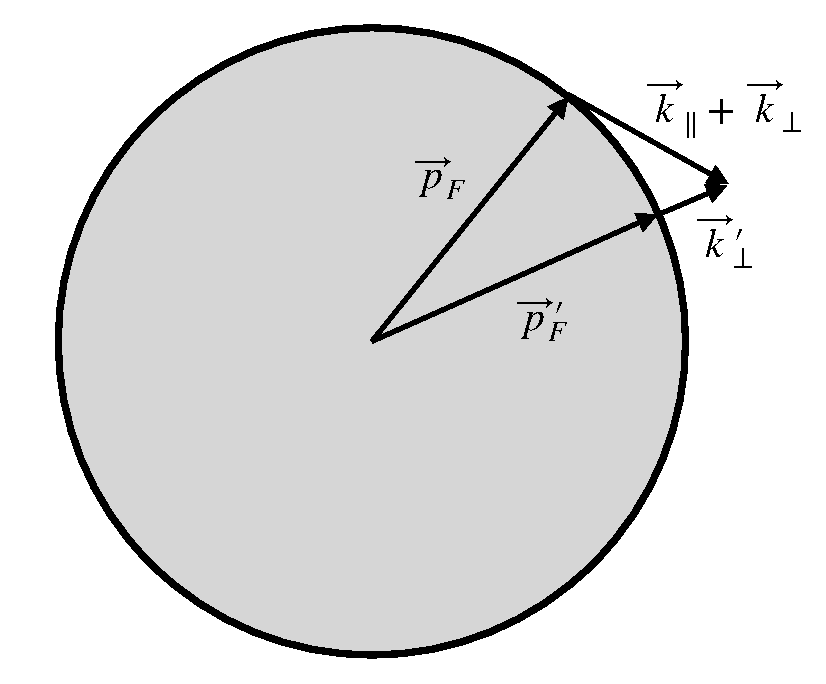
\includegraphics[scale=0.4]{imgs/fermi_surface_sphere}
	\end{center}
	\vspace{-.6cm}
\caption{\small Fermi面に平行な運動量と垂直な運動量。} \label{fig: Fermi surface}
\end{figure}

主要な運動項を決定したので、このEFTのパワーカウンティング則を導ける。まず、不変な微分演算子が一様にスケールするためには、次が必要である。
%
\begin{align} \label{fermi liquids power counting rule 1}
	\vec v_F \cdot \vec \nabla \sim \d_t \sim \epsilon.
\end{align}
%
運動項が決定するのは、空間勾配の一成分、すなわちFermi面に垂直な成分のスケーリングだけである。これは、これまでに考えた他のすべてのモデルとは異なる。その理由を理解するため、各Fourierモード$\psi_{{\vec p}_F} (t , \vec k)$の運動量$\vec k$を、$\vec p_F$におけるFermi面に平行な方向と垂直な方向に分解しよう。
%
\begin{align}
	\vec k = \hat v_F (\hat v_F \cdot \vec k ) + \hat v_F \times ( \vec k \times \hat v_F) \equiv \vec k_\perp + \vec k_\parallel \ .
\end{align}
%
すると、図\ref{fig: Fermi surface}に示すように、場のラベルを再定義することで、Fermi面に平行な運動量成分は常に吸収できる。より正確には、Fermi球面上の異なる点における場のFourierモードの間には、次の関係が成り立つ。
%
\begin{align}
	\psi_{\vec p_F} (t, \vec k_\parallel + \vec k_\perp) = \psi_{\vec p_F^{\, \prime}} (t, \vec k_\perp^{\, \prime}), 
\end{align}
%
ただし、各量は次のように与えられる。
%
%
\begin{align}
	k_\perp' = | \vec p_F + \vec k_\parallel + \vec k_\perp|, \qquad \qquad \hat k_\perp' = \hat p_F' = \frac{\vec p_F + \vec k_\parallel + \vec k_\perp}{| \vec p_F + \vec k_\parallel + \vec k_\perp|} \ .
\end{align}
%
したがって、場$\psi_{\vec p_F}$はFermi面に垂直な方向の運動量だけをもつと常に仮定できる。よって、積分測度と場は
%
\begin{align} \label{fermi liquids power counting rule 2}
	dt\,  d^3 x \sim d t \, d x_\perp d^2 x_\parallel \sim \epsilon^{-2}, \qquad \qquad \psi_{\vec p_F} \sim \epsilon^{1/2}, 
\end{align}
%
とスケールしなければならない。これによって、運動項\eqref{S kin fermi liquids}が微分展開において$\mathcal{O}(1)$であることが保証される。

パワーカウンティング則\eqref{fermi liquids power counting rule 1}と\eqref{fermi liquids power counting rule 2}が得られたので、準粒子間の相互作用を論じることができる。まず、原理的には、書き下せる関連な2次項が一つあることに注意しよう。それは
%
\begin{align} \label{quadratic int fermi liquids}
	-  \sum_{\vec p_F} \int dt \, d^3 x \, \Delta \, \psi_{\vec p_F}^\dag  \psi_{\vec p_F} \sim \epsilon^{-1} , 
\end{align}
% 
である。ここで、$\Delta$は、ブースト不変性を保つために$\vec p_F$に依存してはならないパラメータである。この項はエネルギーギャップを加えることによって、準粒子の分散関係を$\epsilon \to \vec v_F \cdot \vec k + \Delta$と変更する。言い換えると、この演算子はすべての準粒子のエネルギーを一定量だけシフトさせる。このようなシフトは常にFermi面の再定義に吸収できる。そのため、2次演算子\eqref{quadratic int fermi liquids}は、場の位相を$\psi_{\vec p_F}' \equiv e^{i \Delta t} \psi_{\vec p_F}$と再定義することによって、常に取り除ける。

さらに興味深いのは、模式的に次の形をもつ4次の周辺的相互作用が存在することである。
%
\begin{align} \label{fermi liquids marginal interactions}
	S_{\rm int} = \sum_{\vec p_{F, i}}{\vphantom{\sum}}' \int dt \, d^3 x \,  g \,  \psi_{- \vec p_{F,3}}^\dag   \psi_{\vec p_{F,1}}  \, \psi_{- \vec p_{F,4}}^\dag \psi_{\vec p_{F,2}} \sim 1 \ ,
\end{align}
%
ここで、総和のプライムは、並進不変性が課す制約$\vec p_{F,1} +   \vec p_{F,2} + \vec p_{F,3} +\vec p_{F,4} = 0$を表している。さらに、係数$g$は、すべてのスピノル添字が$SU(2)$不変な形で縮約されるような添字構造をもち、回転不変性およびブースト不変性と両立する最も一般的な仕方で、ラベル$\vec p_{F, i}$に依存してよい。
%
\begin{figure}[t]
	\begin{center}
		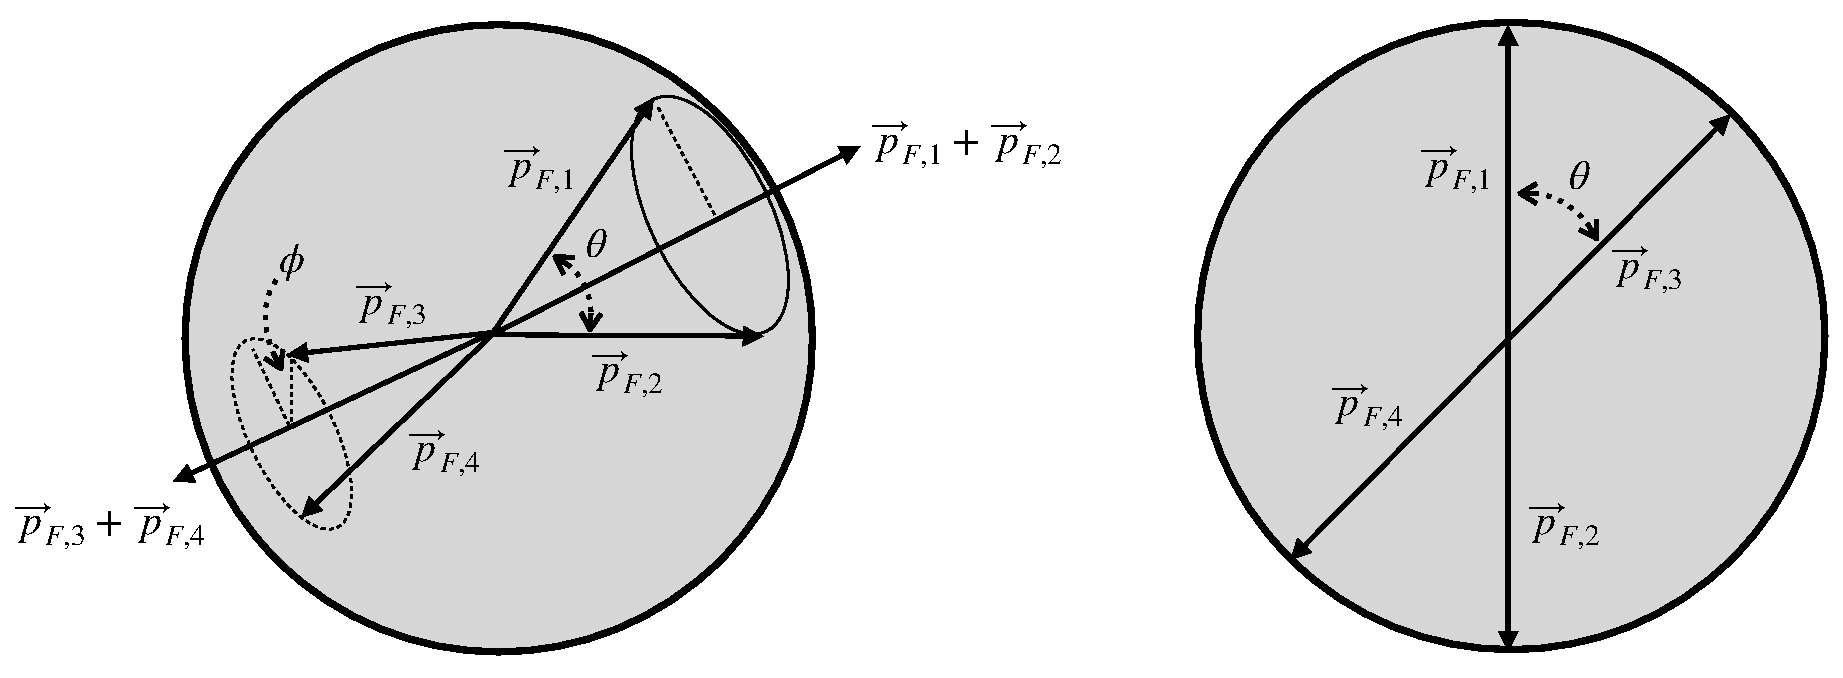
\includegraphics[scale=0.4]{imgs/scattering}
	\end{center}
	\vspace{-.6cm}
\caption{\small Fermi面上で運動量を保存する相互作用。} \label{fig: scattering Fermi surface}
\end{figure}
%

まず、運動量依存性を論じよう。すべての$\vec p_{F,i}$が同時にFermi面上になければならないので、並進不変性の要請は特に厳しい制約となる。これを見るために、運動量空間の任意の二方向に沿って$\vec p_{F,1}$と$\vec p_{F,2}$を選ぼう。この二つのベクトルは、図\ref{fig: scattering Fermi surface}の右図に示すように、$\vec p_{F,1} + \vec p_{F,2}$の方向を軸とする円錐上にある。運動量保存は、$\vec p_{F,3}$と$\vec p_{F,4}$が、同じ軸をもち、原点に対して反対向きの円錐上にあることを要求する。全体の回転を除けば、この配置は二つの角度、すなわち$\vec p_{F,1}$と$\vec p_{F,2}$の間の角度$\theta$、および$\vec p_{F,1}, \vec p_{F,2}$の張る平面と$\vec p_{F,3}, \vec p_{F,4}$の張る平面の間の角度$\phi$だけで完全に記述される。文献~\cite{Shankar:1993pf}に従い、この運動量配置を\emph{零音波チャネル}と呼ぶ。

このチャネルは、$p_{F,1} = - \vec p_{F,2}$という特殊な場合には明確に定義できなくなる。このとき、運動量保存から$p_{F,3} = - \vec p_{F,4}$となる。これらの「背中合わせ」の相互作用は、図\ref{fig: scattering Fermi surface}の右図に示すように、一つの角度$\theta$で特徴付けられる。この種の相互作用を\emph{BCSチャネル}と呼ぶ。
%
\begin{eBox}
%
{\bf 演習4.5：}零音波チャネルの角度$(\theta,\phi)$とBCSチャネルの角度$\theta$を、ラベル$\vec p_{F,i}$を用いて表せ。
%
\end{eBox}
%
次に、BCSチャネルに対象を絞ろう。この場合、4次相互作用は次の形をとる。
%
\begin{align}
	S_{\rm BCS} = \sum_{\vec p,\vec p^{\, \prime}} \int dt \, d^3 x \,  g_{abcd} (\theta)  \psi_{\vec p^{\, \prime}}^{a \dag}   \psi_{\vec p}^b  \, \psi_{- \vec p^{\, \prime}}^{c\dag} \psi_{- \vec p}^d \ ,
\end{align}
%
ここで、$\theta$は$\vec p$と$\vec p^{\, \prime}$の間の角度である。$SU(2)$スピン対称性が許す独立な添字構造は二つだけであり、次のように書けることは容易に確かめられる。
%
\begin{align} \label{BCS channel tensor structure}
	g^{abcd} (\theta) &= g_1 (\theta) \, \delta^{ab} \delta^{cd} + g_2	 (\theta) \, \vec \sigma^{ab} \cdot \vec \sigma^{cd} \ . 
\end{align}
%
関数$g_i(\theta)$はさらにLegendre多項式に分解でき、これによって無限個の結合定数$g_{i, \ell}$が実質的に導入される。
%
\begin{align}
	g_i (\theta) = \sum_{\ell} g_{i,\ell} P_\ell (\cos \theta) \ .
\end{align}
%
一見すると、これは、展開パラメータの任意の固定次数において作用に現れる結合定数は有限個であるべきだという、EFTに関する標準的な通念に反するように見える。これは、その通念が、EFTに含まれる場の数は有限であるという暗黙の仮定に基づいているためである。今回の場合、$\psi$を無限個の場$\psi_{\vec p}$に実質的に置き換えている。しかし、予言能力は失われないことに注意しよう。$\theta$の値を固定すると、結合$g_i (\theta)$は、「ソフト」な運動量$\vec k$の運動学的配置が任意である過程を記述する。

% 
\begin{eBox}
%
{\bf 演習4.6：}演習4.5で導いた結果を用いて、零音波チャネルの角度がパリティ変換の下で$(\theta, \phi) \to (\theta, \pi+ \phi)$と変換することを示せ。次に、理論がパリティ不変ならば、零音波チャネルで可能なテンソル構造も式\eqref{BCS channel tensor structure}の形に限られることを示せ。
%
\end{eBox}
%

以上から、フェルミオンが有限密度で存在すると、真空の場合に比べてパワーカウンティング則が大きく変わり、式\eqref{fermi liquids marginal interactions}の形の周辺的相互作用が存在できることが分かった。これらの相互作用は零音波とBCSという二つのチャネルに分けられ、原理的には無限個の結合で記述される。通常どおり、量子補正により、結合の異常次元に応じて、これらの相互作用は関連にも非関連にもなりうる。引力的な相互作用は関連となり、斥力的な相互作用は非関連となることが分かっている~\cite{Shankar:1993pf}。

ある系において結合が正か負かは、実験を行うか、基礎となるUV理論にマッチングすることによってしか決定できない。そのUV理論の結合は、別の実験によって決定されていなければならない。しかし、一般論として、関連となる結合は低エネルギーで顕著な現象を生み出すと期待できる。例えば、ヘリウム3では$\ell =1$のBCSチャネルの結合が周辺的に関連であり、そのためヘリウム原子が対を作って低温で凝縮し、超流動が生じる。一方、金属では$\ell =0$のBCSチャネルが関連となり、通常の超伝導を引き起こす。これらの現象を詳しく論じることは本講義の範囲を大きく超えるが、関心のある読者のために、この節の最後に有用な資料をいくつか挙げてある。全体を通じて、Fermi液体論も他のEFTと同じく、自由度、展開パラメータ、対称性の特定の選択に基づいていることが伝われば幸いである。このわずかな仮定だけから、数多くの興味深い物理が導かれる。




\subsectionlink{非相対論的QED}


次に、少し複雑な例である非相対論的QED（NRQED）を考える。これは、真空中の非相対論的フェルミオンが、式\eqref{S psi}の接触相互作用ではなく、長距離の電磁相互作用を受けるEFTである。これまでに論じたEFTとは異なり、NRQEDには考慮すべき運動学的領域が複数あり、その結果、パワーカウンティングはかなり複雑になる。例えば、NRQEDを用いて、等しい質量の構成粒子からなる束縛状態を研究し、速度$v$のべきによる系統的な展開で観測量を計算できる。\footnote{この節では、再び$c=1$の単位系を用いる。}実際、ビリアル定理と不確定性原理を組み合わせれば、束縛状態では$v$が小さくなければならないことは容易に分かる。
%
\begin{align}
	\frac{m v^2}{2} \sim \frac{\alpha}{r} \lesssim \alpha \, m v \qquad \Longrightarrow \qquad v \lesssim \alpha \ll 1. 
\end{align}
% 
NRQEDの動機は、本講義でこれまでに扱った他のEFTの動機とは異なることを強調しておこう。ここでは、低エネルギーでは生成できないほど重い粒子を積分消去するわけでも、UVにおける強結合の物理や未知の物理の低エネルギーでの帰結をモデル化することが主目的でもない。むしろ、QEDのような十分に理解された摂動的理論を用いて、小さな速度$v$のべきによる展開として観測量を計算することに関心がある。これを最も効率的に実現するには、$v$に関するパワーカウンティングを作用の段階で直接実装できる、NRQEDのようなEFTへ移ればよい。

出発点は、通常のQEDの作用である。
%
\begin{align}
	S = \int d^4 x \left\{ \bar \Psi [i \gamma^\mu (\partial_\mu - i e A_\mu) - m ] \Psi - \frac{1}{4} F_{\mu\nu} F^{\mu\nu} - \frac{1}{2\xi} (\partial_\mu A^\mu)^2 \right\},
\end{align}
%
ここでは、ゲージ固定項をすでに明示的に加えてある。以下では、$\xi = 1$であるFeynmanゲージを用いる。$m$よりもはるかに小さいエネルギーでは、\ref{sec: NR fermions in vacuum}節で行ったのとまったく同じように、フェルミオン場の位相を再定義して反粒子を積分消去できる。$A^\mu = (\Phi, \vec A)$と書くと、次のツリーレベル有効作用を得る。
%
\begin{align} \label{NRQED action}
	S_{\rm eff}^{(0)} = \int dt \, d^3 x \left\{  \psi^\dag \left( i \partial_t  -e \Phi + \frac{\vec{D}^2}{2 m} + \frac{e}{2m} \vec B \cdot \vec \sigma \right) \psi  - \frac{1}{2} \partial_\mu A_\nu \partial^\mu A^\nu + \mathcal{O}(1/m^2) \right\} ,
\end{align}
%
ここで、2成分スピノル$\psi$は式\eqref{2-spinor def}で定義され、電場と磁場は通常どおりスカラーポテンシャルおよびベクトルポテンシャルから定義される~\cite{Jackson:1998nia}。また、$\vec D = \vec \nabla - i e \vec A$である。この作用は、式\eqref{S psi}の作用の接触相互作用を、光子を媒介とする相互作用に置き換えたものに相当する。
%
\begin{eBox}
%
{\bf 演習4.7：}式\eqref{NRQED action}のツリーレベル有効作用を導け。
\end{eBox}
%
$\vec B$に線形な項は、偶発的な$SU(2)$スピン対称性と空間回転を、それらの対角部分群にまで破ることに注意しよう。この項は$\vec \mu \cdot \vec B$という形をもち、$\vec \mu = 2 \mu_B \vec S$は磁気モーメントの密度、$\mu_B = q / (2 m c)$はBohr磁子、$\vec S = \frac{1}{2}\tilde \Psi_-^\dag \sigma^i \tilde \Psi_-$はスピン密度である。すなわち、これは、磁場中の磁気双極子密度のよく知られたポテンシャルエネルギーに負号を付けたものである。

\begin{figure}
	\begin{center}
		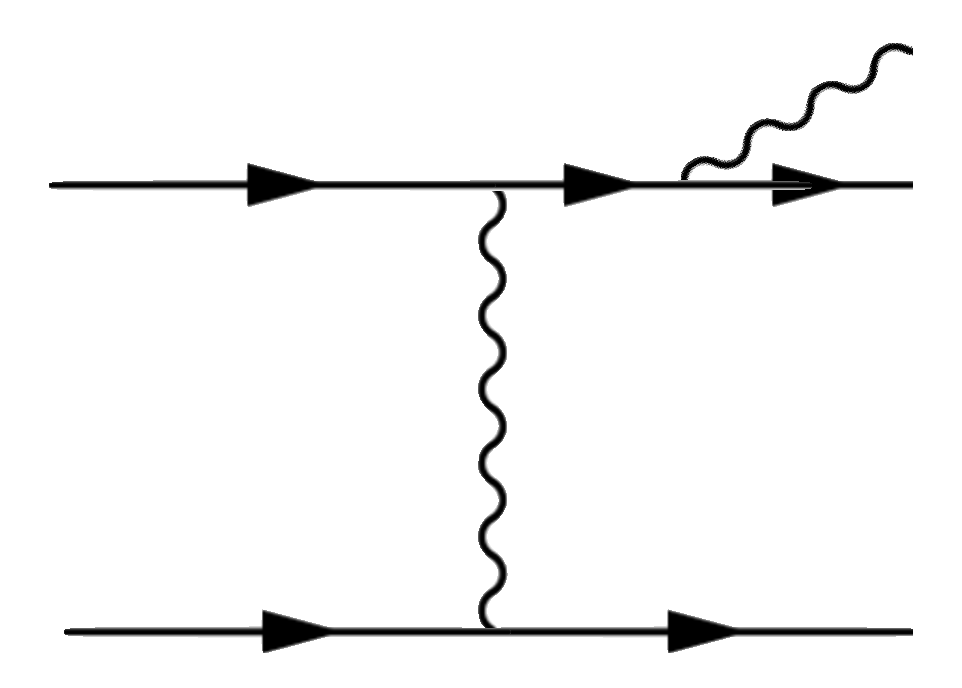
\includegraphics[scale=0.3]{imgs/NRQED}
	\end{center}
	\vspace{-.6cm}
\caption{\small QEDにおけるツリーレベル・ダイアグラムの例。} \label{fig:NRQED}
\end{figure}

ゲージ不変性は、作用\eqref{NRQED action}中の各微分がゲージポテンシャルとともに現れることを要求する。このため、有効作用を$m$の逆べきで展開することが、$p / m = v$のべきで展開することと等価であるかは、もはや明らかではない。等価となるためには、ポテンシャルも$v$のようにスケールする必要がある。これを確認するには、時間微分と空間微分がポテンシャルにどのように作用するかを知る必要がある。そうすれば、運動項が$\mathcal{O}(1)$の量であることを要求して、通常どおり場のスケーリング則を求められるからである。そのために、図\ref{fig:NRQED}のダイアグラムを考えよう。すべてのフェルミオン外線のエネルギーと運動量は$(mv^2, mv)$のオーダーである。したがって、散乱過程で交換され、光子内線によって運ばれるエネルギーと運動量も、一般には$(mv^2, mv)$のオーダーでなければならない。この運動学的領域を\emph{ポテンシャル}領域と呼ぶ。次に、この過程で放出される光子を考えよう。エネルギー保存により、そのエネルギーは高々$\mathcal{O}(mv^2)$である。対応する外線はオンシェルでなければならないので、そのエネルギーと運動量は$(mv^2, mv^2)$のオーダーでなければならない。この運動学的領域を\emph{ウルトラソフト}領域と呼ぶ。\footnote{これは\emph{放射}領域とも呼ばれる。}このことは、$A^\mu$が運ぶ運動量が、Feynmanダイアグラム中で光子の線が果たす役割に依存することを示している。この結果をそのまま受け取ると、ゲージポテンシャルに$v$の明確な次数を割り当てられないように見える。この問題にどう対処し、$v$について明確に定義されたパワーカウンティングを実装するかを、この後に示す。

実は、ポテンシャル領域とウルトラソフト領域だけで話が終わるわけではない。これを見るために、まず少し脇道にそれ、\high{領域展開法}として知られる、もう一つのEFTの手法を論じる必要がある。まず文献~\cite{Griesshammer:1997wz}に従い、簡単な例を用いて導入しよう。次の1次元積分を考える。
%
\begin{align} \label{toy integral regions}
	I(a, b) = \int_{- \infty}^{+\infty}  dk \, \frac{1}{k^2 - a^2+ i \epsilon}\, \frac{1}{k^2 - b^2 + i \epsilon},
\end{align}
%
この構造は、相対論的場の理論に現れるある種の1ループ積分を思い起こさせる。ここでは、二つの極の位置が大きく隔たっている、すなわち$ a / b \ll 1$である状況に関心がある。このとき、$I(a, b)$は小さなパラメータ$a / b$のべきによる展開として計算できる。この積分への支配的な寄与が極の近傍の領域から生じると仮定するのは妥当に思える。そこで、積分全体を、$k= \pm a$の近傍と$k=\pm b$の近傍を中心とする二つの積分の和として近似する。
%
\begin{align}
	I(a, b) \simeq  \left[ \int_{k^2 \sim a^2} dk + \int_{k^2 \sim b^2} dk \right] \, \frac{1}{k^2 - a^2+ i \epsilon}\, \frac{1}{k^2 - b^2 + i \epsilon}. 
\end{align}
%
最初の領域では、被積分関数の第2の因子を$k^2/b^2$のべきで展開できる。一方、二つ目の領域では、第1の因子を$a^2/k^2$のべきで展開でき、その結果、次を得る。
%
\begin{align} \label{toy 2 regions}
	I(a, b) \simeq \sum_{n=0}^\infty \left[ -\frac{1}{b^2}\int_{k^2 \sim a^2} dk  \, \frac{1}{k^2 - a^2+ i \epsilon} \frac{k^{2n}}{b^{2n}}  + \int_{k^2 \sim b^2} \frac{dk}{k^2} \, \frac{1}{k^2 - b^2 + i \epsilon} \frac{a^{2n}}{k^{2n}}  \right]. 
\end{align}
%
これら二つの積分の正確な値は、一般に、$k= \pm a$と$k=\pm b$の近傍の領域をどのように選ぶかに依存する。この点は、ここまで意図的に曖昧にしてきた。ここから行うのは、これら二つの領域を実軸全体に拡張することである。一見すると、これは非常にまずい考えに思えるかもしれない。二つの極から遠く離れたところでは、用いた級数展開が正当化されないように見えるからである。しかも、第1の積分は$n \neq 0$でUV発散するが、式\eqref{toy integral regions}のもとの積分は発散しなかった。しかし、次元正則化を用いれば、この問題には容易に対処できる。すると、実軸全体にわたる二つの積分は厳密に計算でき、次が得られる。
%
\begin{align}
	I(a, b) \simeq \frac{i \pi}{a} \frac{1}{b^2 - a^2} - \frac{i \pi}{b} \frac{1}{b^2 - a^2} = \frac{i \pi}{ab (a+b)}. 
\end{align}
%
驚くべきことが起きた。一見疑わしい中間操作を行ったにもかかわらず、最終結果は単によい近似であるだけでなく、実際に$I(a,b)$の\emph{厳密な}値となったのである。（これは、標準的な複素積分の方法で式\eqref{toy integral regions}の積分を直接計算すれば確かめられる。）積分を実軸全体に拡張しても問題がなかったのは、各極から遠く離れた領域では、被積分関数中のすべてのスケールを無視でき、スケールをもたない積分は次元正則化ではゼロになるからである。

以上により、式\eqref{toy integral regions}の積分は、被積分関数のすべての極を特定し、各極の周りで展開して生じる寄与を足し合わせることで計算できることを示した。この方法は領域展開法と呼ばれ、EFTのループ積分に適用すると非常に有用な道具となる。今回の簡単な例では、この方法が実際に機能することを納得してもらうために、級数を足し合わせて厳密な結果を得た。しかしEFTでは、式\eqref{toy 2 regions}の積分が、小さなパラメータ$a / b$についての展開として明示的に整理されているという点の方に関心がある。

実際、式\eqref{toy integral regions}の被積分関数にある二つの因子を、異なる二つの粒子の伝播関数と考えると、式\eqref{toy 2 regions}には非常に興味深い解釈を与えられる。第1の積分は、一つの伝播関数$1/(k^2 - a^2 + i \epsilon)$、$n$個の静的伝播関数$1/b^2$、および$n$個の場の挿入$k^2$からなるループに等しい。これらは、運動量が$k^2 \sim a^2$の領域にある場に関わる伝播関数および2次の頂点である。第2の積分にも同様の解釈が可能であり、対応する領域は$k^2 \sim b^2$となる。ここから学べるのは、$I(a,b)$を$a/b$のべきによる展開として整理するには、各場が関わる運動学的領域ごとに、その場のコピーを形式的に導入するとともに、それらすべてのコピーの間の相互作用も追加する必要があるということである。

\begin{figure}
	\begin{center}
		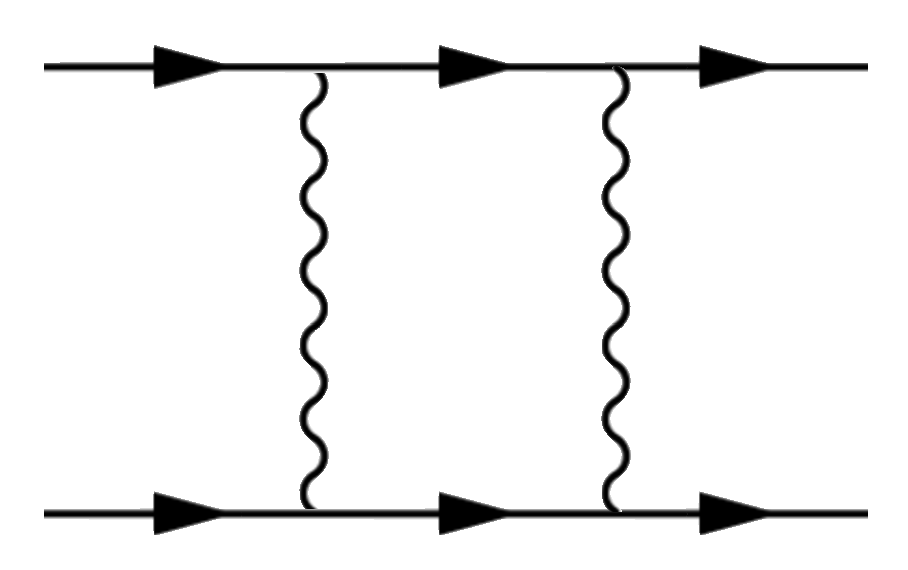
\includegraphics[scale=0.3]{imgs/NRQEDbox}
	\end{center}
	\vspace{-.6cm}
\caption{\small QEDにおける1ループ・ダイアグラムの例。} \label{fig:NRQEDbox}
\end{figure}


ここでNRQEDの議論に戻り、この考えを実際にどう実装するかを見てみよう。NRQEDで役割を果たす運動学的領域として、ポテンシャル領域とウルトラソフト領域の二つをすでに特定したが、実はさらにもう一つ考慮すべき領域がある。例えば、図\eqref{fig:NRQEDbox}に示したQEDのループ・ダイアグラムを考えよう。重心系で計算し、外線のフェルミオンがすべて非相対論的である状況に関心を絞る。全体にかかる定数因子を除くと、このループ・ダイアグラムは次の積分に等しい。
%
{\allowdisplaybreaks[0]\begin{align}
	& \int \frac{d^4 k}{(2\pi)^4} \,  N \, \frac{1}{k_0^2 - \vec{k}^{ 2} + i \epsilon } \, \frac{1}{(p_0 +k_0 - p_0')^2- (\vec p + \vec k - \vec{p}^{\,\prime})^2+ i \epsilon } \nonumber \\ 
	& \qquad \qquad \qquad \qquad \frac{1}{(p_0-k_0)^2 - (\vec p + \vec k)^2 - m^2 + i \epsilon } \, \frac{1}{(p_0+k_0)^2 - (\vec p + \vec k)^2- m^2 + i \epsilon   }, 
\end{align}}
%
ここで、$\pm \vec p$（$\pm \vec p^{\, \prime}$）は入射粒子（出射粒子）の3運動量であり、$N$は運動量の解析関数で、この議論では役割を果たさない。フェルミオンの運動エネルギー$E = p^0 - m$を用いて被積分関数を書き換え、記法を簡単にするために$i\epsilon$の因子を省くと便利である。その結果は次のとおりである。
%
\begin{align}
	& \int \frac{d^4 k}{(2\pi)^4} \,  N \, \frac{1}{k_0^2 - \vec{k}^{ 2} + i \epsilon } \, \frac{1}{(E - E' +k^0)^2- (\vec p + \vec k - \vec{p}^{\,\prime})^2+ i \epsilon } \nonumber \\ 
	& \qquad \qquad \qquad \qquad \qquad \qquad \frac{1}{E^2 - 2E k^0 - (\vec p + \vec k)^2 + i \epsilon } \, \frac{1}{E^2 + 2 E k^0 - (\vec p + \vec k)^2+ i \epsilon   }.
\end{align}
%
先ほどの議論によれば、被積分関数の任意の極の位置は、考慮すべき運動学的領域に対応する。$E, E' \sim mv^2$、$p, p' \sim mv$なので、第2の伝播関数は$(k^0, \vec k) \sim (mv, mv)$に極をもつ。この領域を\emph{ソフト}領域と呼ぶ。光子内線がソフトな4運動量を運ぶときには、エネルギー保存により、フェルミオン内線も同様でなければならないことに注意しよう。ソフト領域が必要となるのは、量子ループを考慮するときだけである。実際、\emph{古典的}な重力束縛状態を扱う非相対論的一般相対論（NRGR）~\cite{Goldberger:2007hy,Porto:2016pyg}では、この領域は何の役割も果たさない。

NRQEDで速度展開を系統的に実装するには、ソフト、ポテンシャル、ウルトラソフトの三つの領域で十分であることが分かる。このため、場$\psi$と$A^\mu$を次のように分解する。
%
\begin{subequations}\label{psi A decomposition}
\begin{align} 
	\psi &= \psi_{\rm S} + \psi_{\rm P} \\ 
	A^\mu &= A^\mu_{\rm S} + A^\mu_{\rm P} + A^\mu_{\rm U},
\end{align}
\end{subequations}
%
ここで、添字は対応する領域を表している。ウルトラソフトなフェルミオンを導入する必要がないことに注意しよう。上で導入したさまざまな場の間の相互作用は、$\mathcal{O} (mv^2)$の精度でエネルギーと運動量を保存しなければならない。ソフト領域とポテンシャル領域の場は$\mathcal{O}(mv)$のエネルギーまたは運動量をもつため、この段階では、それをどう実装するかは明らかでない。さらに、異なる領域の場の間の相互作用について、どのようにパワーカウンティングを行うべきかも明らかでない。積分測度$d^4x$は、どのようにスケールすべきなのだろうか。これらの問題に対処するため、ソフト場とポテンシャル場の位相を再定義し、$\mathcal{O}(mv)$の位相を取り出すことができる。
%
{\allowdisplaybreaks[0]\begin{subequations} \label{NRQED rephasing}
\begin{align}
	\psi_{\rm S} (x) &= \sum_p e^{i p \cdot x} \, \psi_{{\rm S}, p} (x) \\
	A_{\rm S}^\mu (x) &= \sum_p e^{i p \cdot x} \, A_{{\rm S}, p}^\mu (x) \\
	\psi_{\rm P} (x) &= \sum_{\vec p} e^{i \vec p \cdot \vec x} \, \psi_{{\rm P}, \vec p} \, (x) \\
	A_{\rm P}^\mu (x) &= \sum_{\vec p} e^{i \vec p \cdot \vec x} \, A_{{\rm P}, \vec p}^\mu \, (x) . 
\end{align}
\end{subequations}}
% 
ソフト場からは4運動量を、ポテンシャル場からは3運動量を取り出したことに注意しよう。上で述べた手順は、複数の領域の存在を考慮する必要があることを除けば、式\eqref{Psi tilde def}でフェルミオン場$\psi$を多くの場$\psi_{\vec p_F}$の和として表したときの手順と大きくは違わない。なお、ソフト場とポテンシャル場からソフトな位相を取り出すことは、ある種の多重極展開と考えることもできる~\cite{Labelle:1996en,Grinstein:1997gv}。ウルトラソフト場は、ソフト場とポテンシャル場の長波長での振る舞いしか探れないので、これは直観的にも理解できる。

\begin{table}[t!]
  \begin{center}
    \caption{NRQEDの場とその性質。}
    \label{tab: NRQED}
    \vspace{.4cm}
    \begin{tabular}{cccc}
    	\toprule
      \textbf{領域} & \textbf{場} & \textbf{スケーリング} & \textbf{伝播関数} \\
      	\midrule
      ソフト & $\begin{array}{c}
      		\psi_{{\rm S},  p} \\
      		A_{{\rm S}, p}^\mu 
      	\end{array}$ \vspace{.2cm} & $\begin{array}{l}
      		v^{3/2} \\
      		v 
      	\end{array}$ & $\begin{array}{c}
      		 i /(p^0 - i \epsilon) \\
      		-i \eta^{\mu\nu} / (p^{\, 2} - i \epsilon)
      	\end{array}$ \\
      	\midrule
      ポテンシャル & $\begin{array}{c}
      		\psi_{{\rm P}, \vec p} \\
      		A_{{\rm P}, \vec p}^\mu 
      	\end{array}$ \vspace{.2cm} & $\begin{array}{l}
      		v^{3/2} \\
      		v^{3/2}
      	\end{array}$ & $\begin{array}{c}
      		 i /(k^0 - \vec{p}^{\, 2}/2m + i \epsilon) \\
      		-i \eta^{\mu\nu} / (\vec{p}^{\, 2}  - i \epsilon)
      	\end{array}$ \\
      	\midrule
      ウルトラソフト & $A_{{\rm U}}^\mu$ & $\!\!\!\! v^2$ & $-i \eta^{\mu\nu}/(k^2-i\epsilon)$ \\
      \bottomrule
    \end{tabular}
  \end{center}
\end{table}

式\eqref{psi A decomposition}と\eqref{NRQED rephasing}を有効作用\eqref{NRQED action}に代入すれば、場$\psi_{{\rm S}, p}, \psi_{{\rm P}, \vec p}, A_{{\rm S}, p}^\mu, A_{{\rm P}, \vec p}^\mu \, ,$および$A_{{\rm U}}^\mu$の支配的な運動項と、それらの相互作用を導ける。これらの場に含まれるのは、残余のエネルギーと運動量が$\mathcal{O}(mv^2)$であるFourierモードだけなので、$\mathcal{O}(mv^2)$の精度での4運動量保存は自動的に保証される。さらに、積分測度の適切なスケーリングは、今や明らかに$d^4x \sim 1/v^8$である。すると、各場が$v$に応じてどうスケールするかを求め、伝播関数を計算することは容易である。結果を表\ref{tab: NRQED}にまとめた。ここでは、ソフトな運動量、すなわちラベルとしての運動量を$p$で、ウルトラソフトな運動量、すなわち残余運動量を$k$で表している。特に、ウルトラソフトなゲージ場は偏微分と同じようにスケールし、どちらも$\mathcal{O} (mv^2)$であることに注意しよう。したがって、これらを用いて、一様にスケールする共変微分$D_\mu = \partial_\mu - i e A_\mu^{\rm U}$を構成できる。
 
%
\begin{eBox}
%
{\bf 演習4.8：}表\ref{tab: NRQED}にまとめた結果を導け。
\end{eBox}
% 
NRQEDのすべてのFeynman則や実際の応用を詳しく説明することは、領域展開法の導入を主目的としたこの節の範囲を超える。詳しくは、次の節に挙げる文献を参照してほしい。
  



\subsectionlink{さらに学ぶための文献}



Fermi液体のEFTに関する標準的な文献は、PolchinskiのTASI講義録~\cite{Polchinski:1992ed}である。繰り込み群に基づく、有限密度フェルミオンのより網羅的な扱いについては、文献~\cite{Shankar:1993pf}を参照されたい。ヘリウム3の超流動に関する初期の教育的なレビューとして、文献~\cite{Leggett:1975te}がある。束縛状態の研究にNRQEDを用いることが最初に提唱されたのは、文献~\cite{Caswell:1985ui}である。非相対論的ゲージ理論のパワーカウンティングに伴う複雑さの大部分は、非相対論的QCD（NRQCD）の文脈で整理されてきた。NRQCDの詳細については、例えば文献~\cite{Rothstein:2003mp,Griesshammer:1997wz}を参照されたい。また、NRQEDに基づくLambシフトの計算も、文献~\cite{Rothstein:2003mp}にある。

\newpage


\section*{謝辞}


本講義を行う機会を与えてくださった第2回Joint ICTP-Trieste/ICTP-SAIFR school on Particle Physicsの主催者、Enrico Bertuzzo、Joan Elias Mir\'o、Rogerio Rosenfeld、Giovanni Villadoroに感謝する。また、刺激的な議論を交わしてくださったすべての参加者と他の講師にも感謝する。本講義録の準備にあたっては、この主題に関する多くの優れたレビューを読むことで多大な恩恵を受けた。その大部分は、適切な箇所で引用している。また、有益な議論と本講義録の初期稿へのコメントをくださったAngelo Esposito、Walter Goldberger、Garrett Goon、Alberto Nicolis、Rachel Rosen、Adam Solomon、そして特にIra Rothsteinに感謝する。本研究は、National Science Foundationの助成金No. PHY-1915611による支援を一部受けた。

